\chapter{SIMULATING THE MOTION OF ROBOT}
    \section{Topic}
    Simulate the motion of this robot to plot initial letters from the first names of your team members on a certain plane that is perpendicular to axis \( z_0 \).
    \section{Theory}
        Simulate robot in simscape $(\theta_1, d_2, \theta_4)$ change from $(0,2200, 0)$ to $(90^{\circ}, 2700, 90^{\circ})$.
        \begin{figure}[H]
            \centering
            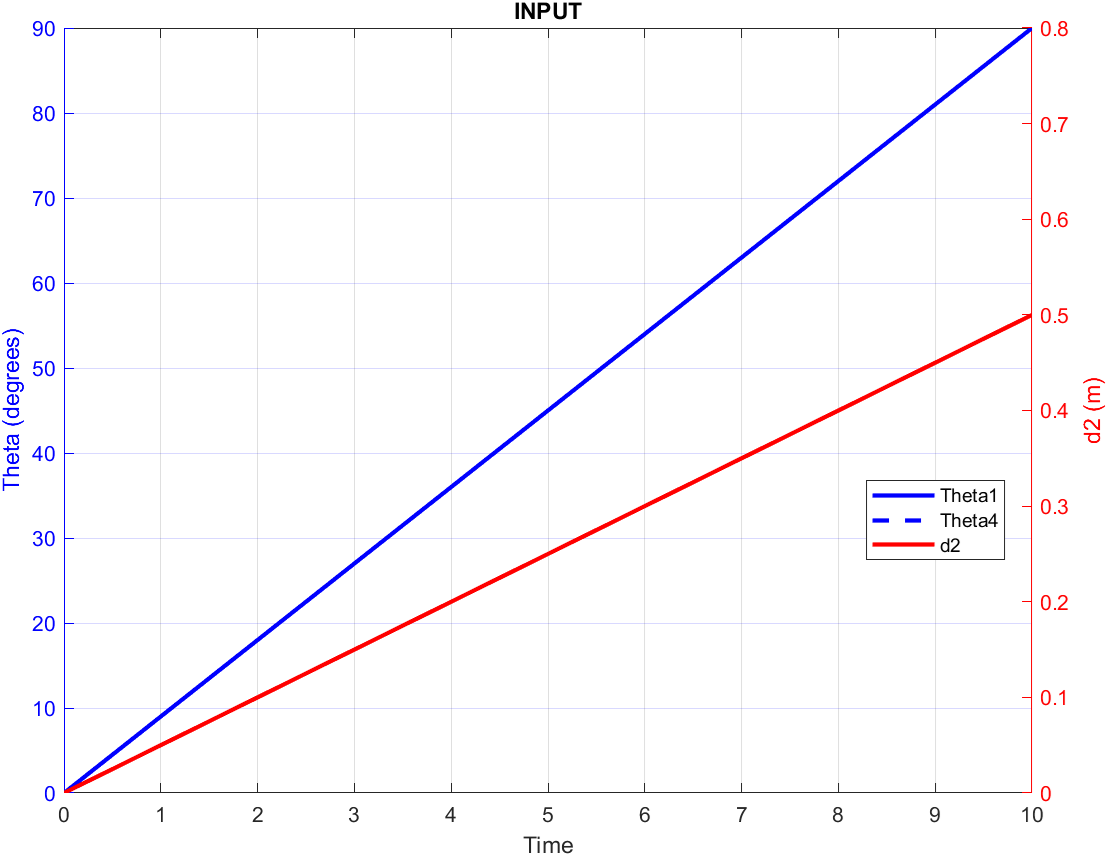
\includegraphics[width=0.8\textwidth]{pictures/theta_d_change.png}
            \caption{Simulation of the robot}
            \label{fig:theta_d_change}
        \end{figure}
        Apply to forward, get position of end-effector \( (x,y,z) \) with respect to time \( t \)
        \begin{figure}[H]
            \centering
            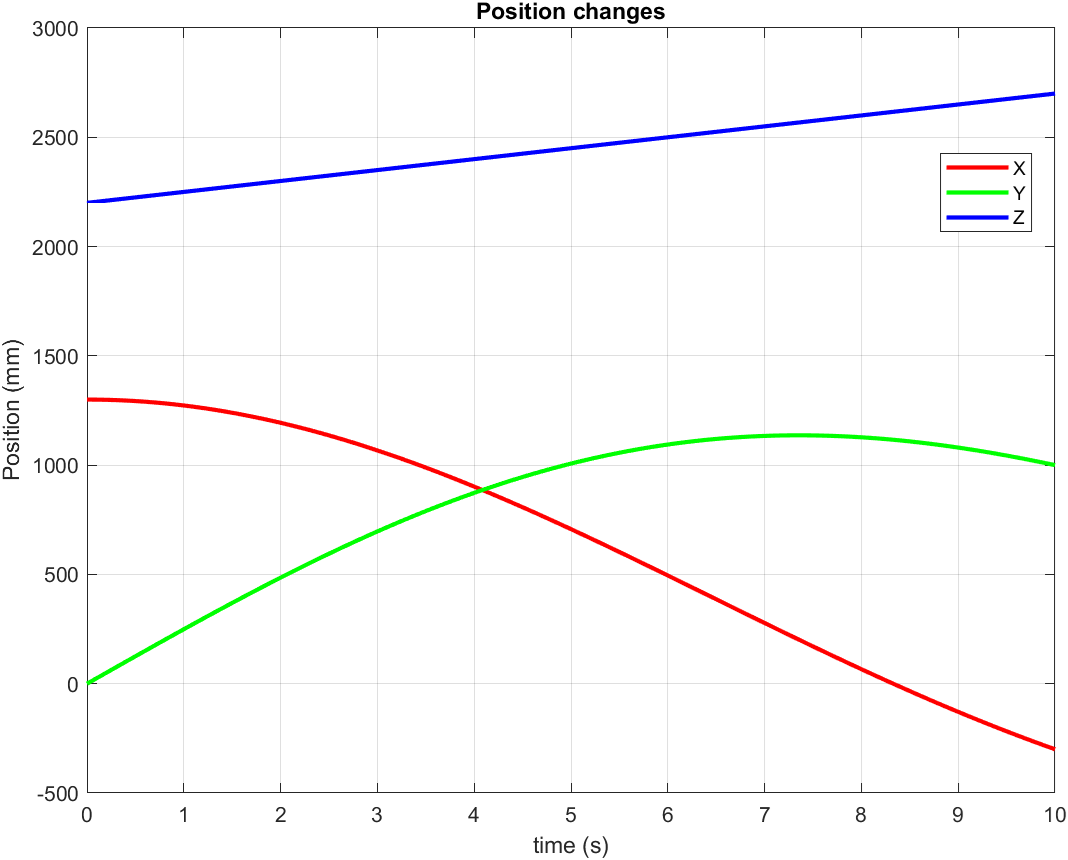
\includegraphics[width=0.8\textwidth]{pictures/test_forward.png}
            \caption{Simulation of the robot}
            \label{fig:test_forward}
        \end{figure}

        
    \section{Application}
    Modeling robot by Solidworks then convert to step file, this is suitable for Simscape 
    Multibody Link.
    \begin{figure}[H]
        \centering
        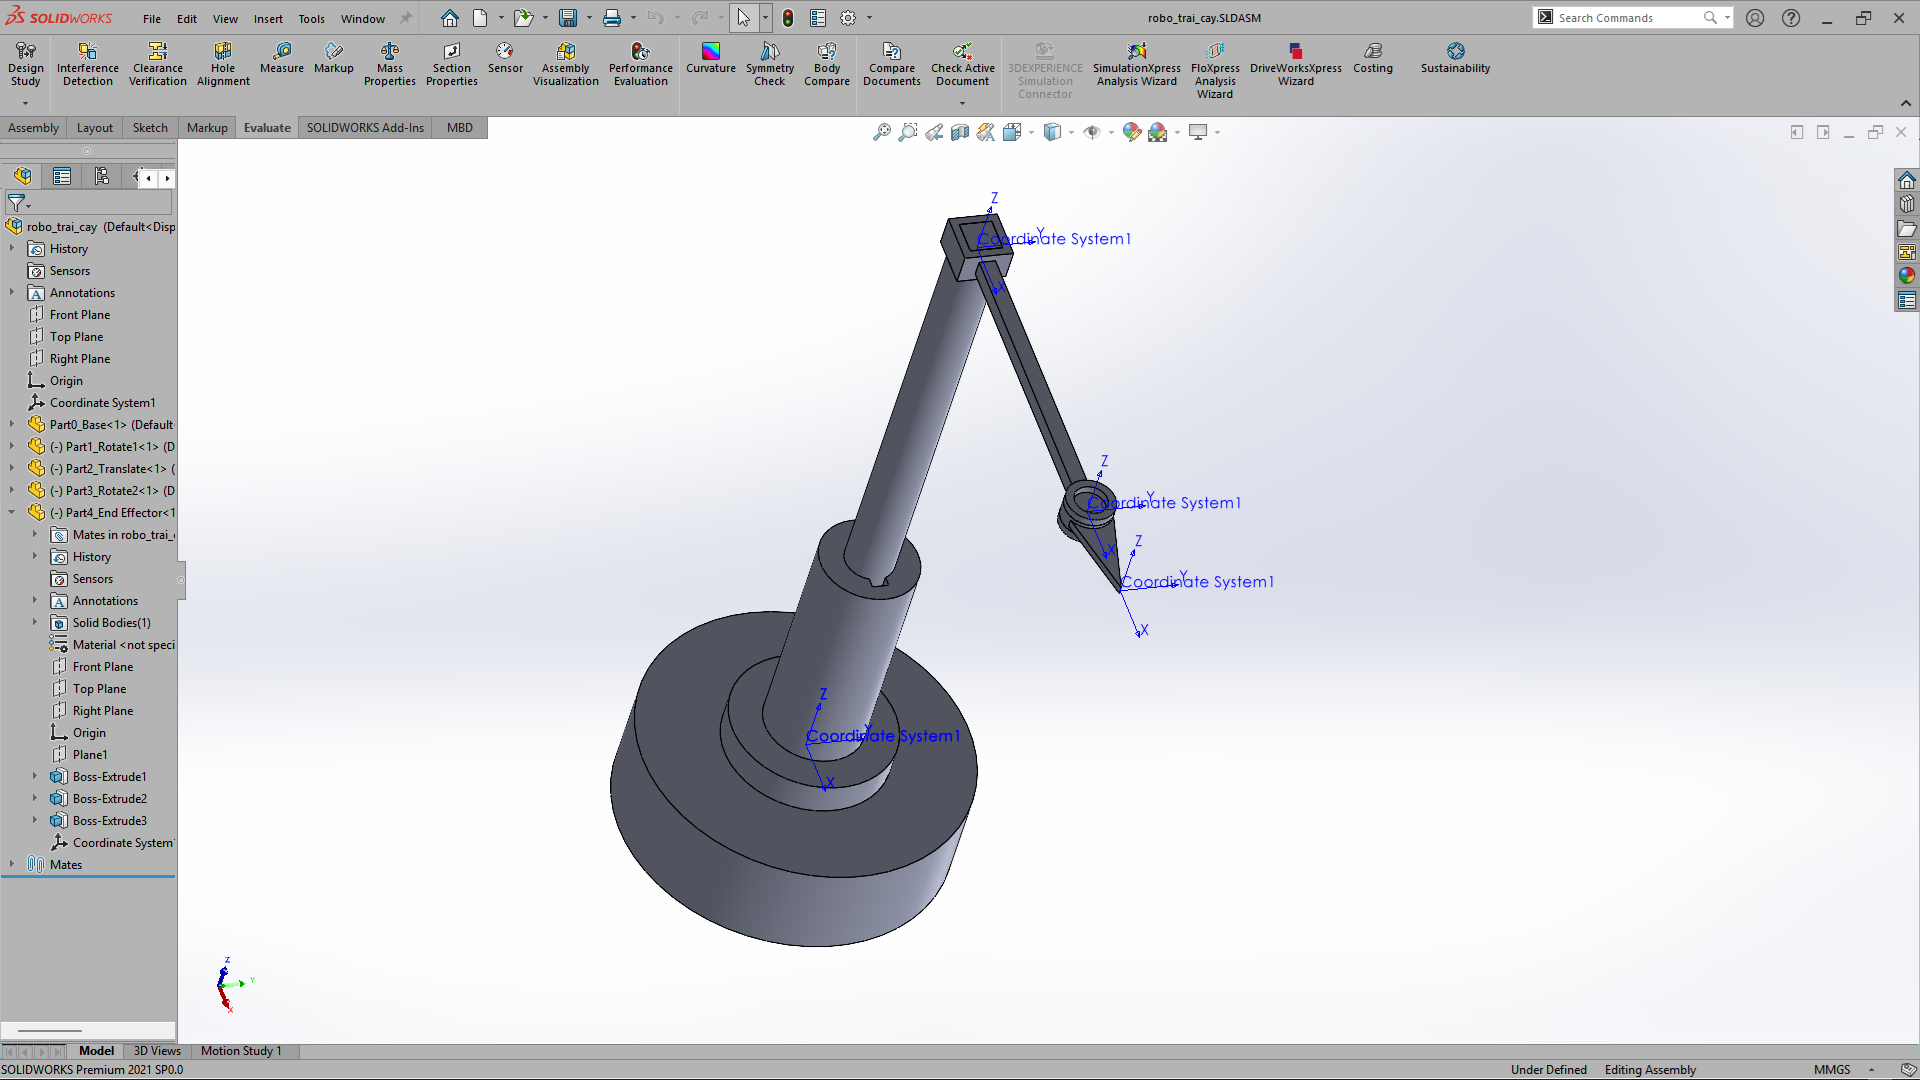
\includegraphics[width=0.8\textwidth]{pictures/solid.png}
        \caption{Robot model in Solidworks}
        \label{fig:robot_model}
    \end{figure}
    Model in Simscape Multibody Link
    \begin{figure}[H]
        \centering
        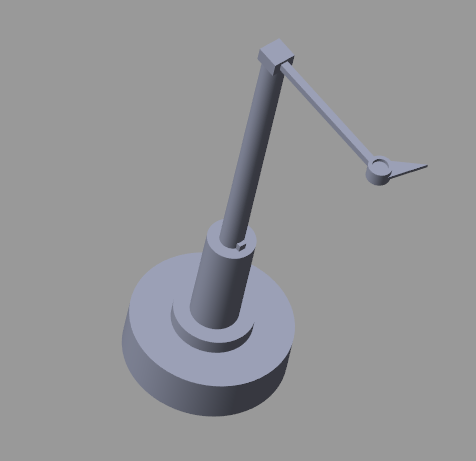
\includegraphics[width=0.6\textwidth]{pictures/simscape.png}
        \caption{Robot model in Simscape Multibody Link}
        \label{fig:simscape_model}
    \end{figure}
    Block diagrams of Matlab Simulink is as the follow:
    \begin{figure}[H]
        \centering
        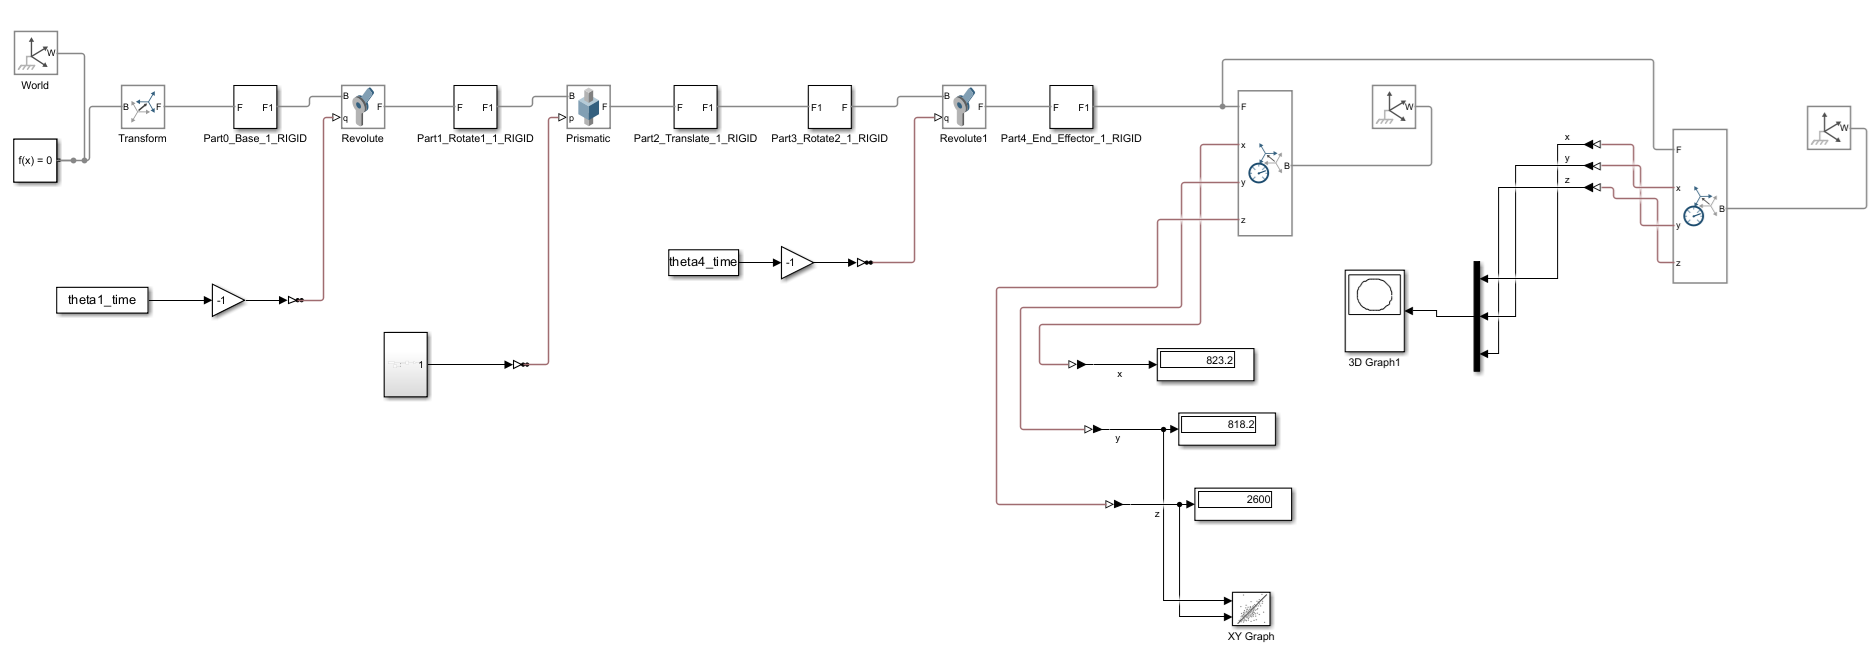
\includegraphics[width=1\textwidth]{pictures/simulink.png}
        \caption{Block diagram of Matlab Simulink}
        \label{fig:simulink_block_diagram}
    \end{figure}
    Results of simulation: \\
    \hspace*{0.6cm}Position \( (x,y,z) \) of robot from transsform sensor
    \begin{figure}[H]
        \centering
        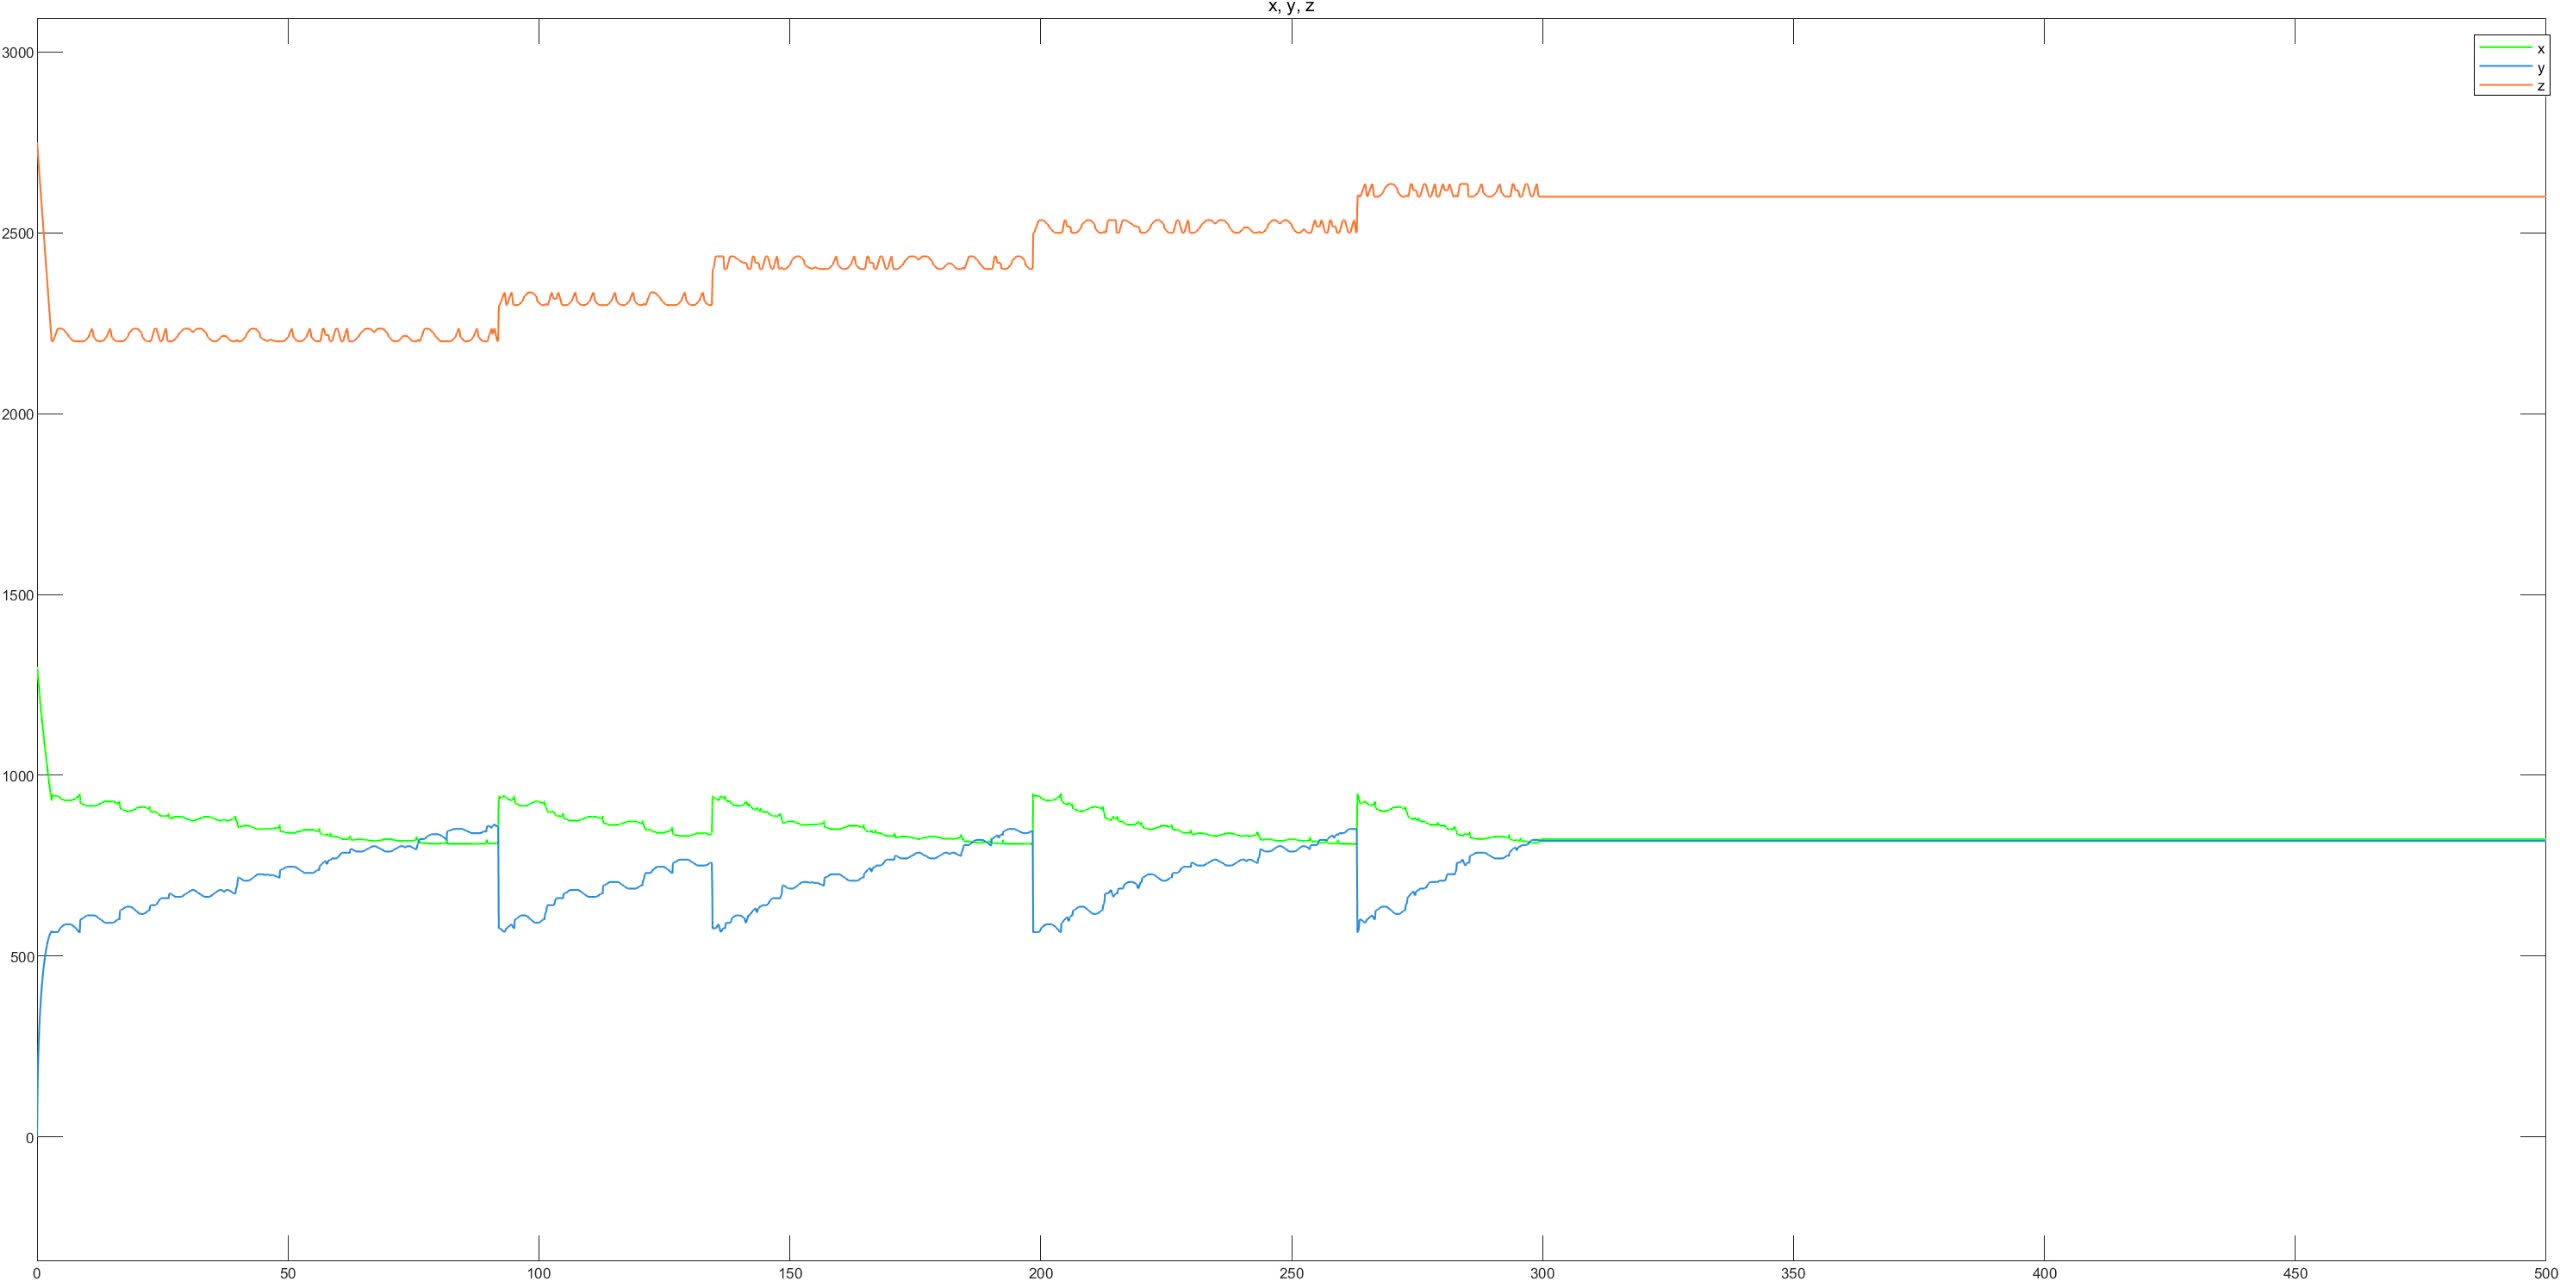
\includegraphics[width=1\textwidth]{pictures/xyz_pos_sensor.png}
        \caption{Position of robot}
        \label{fig:position}
    \end{figure}
    Result on YZ plane
    \begin{figure}[H]
        \centering
        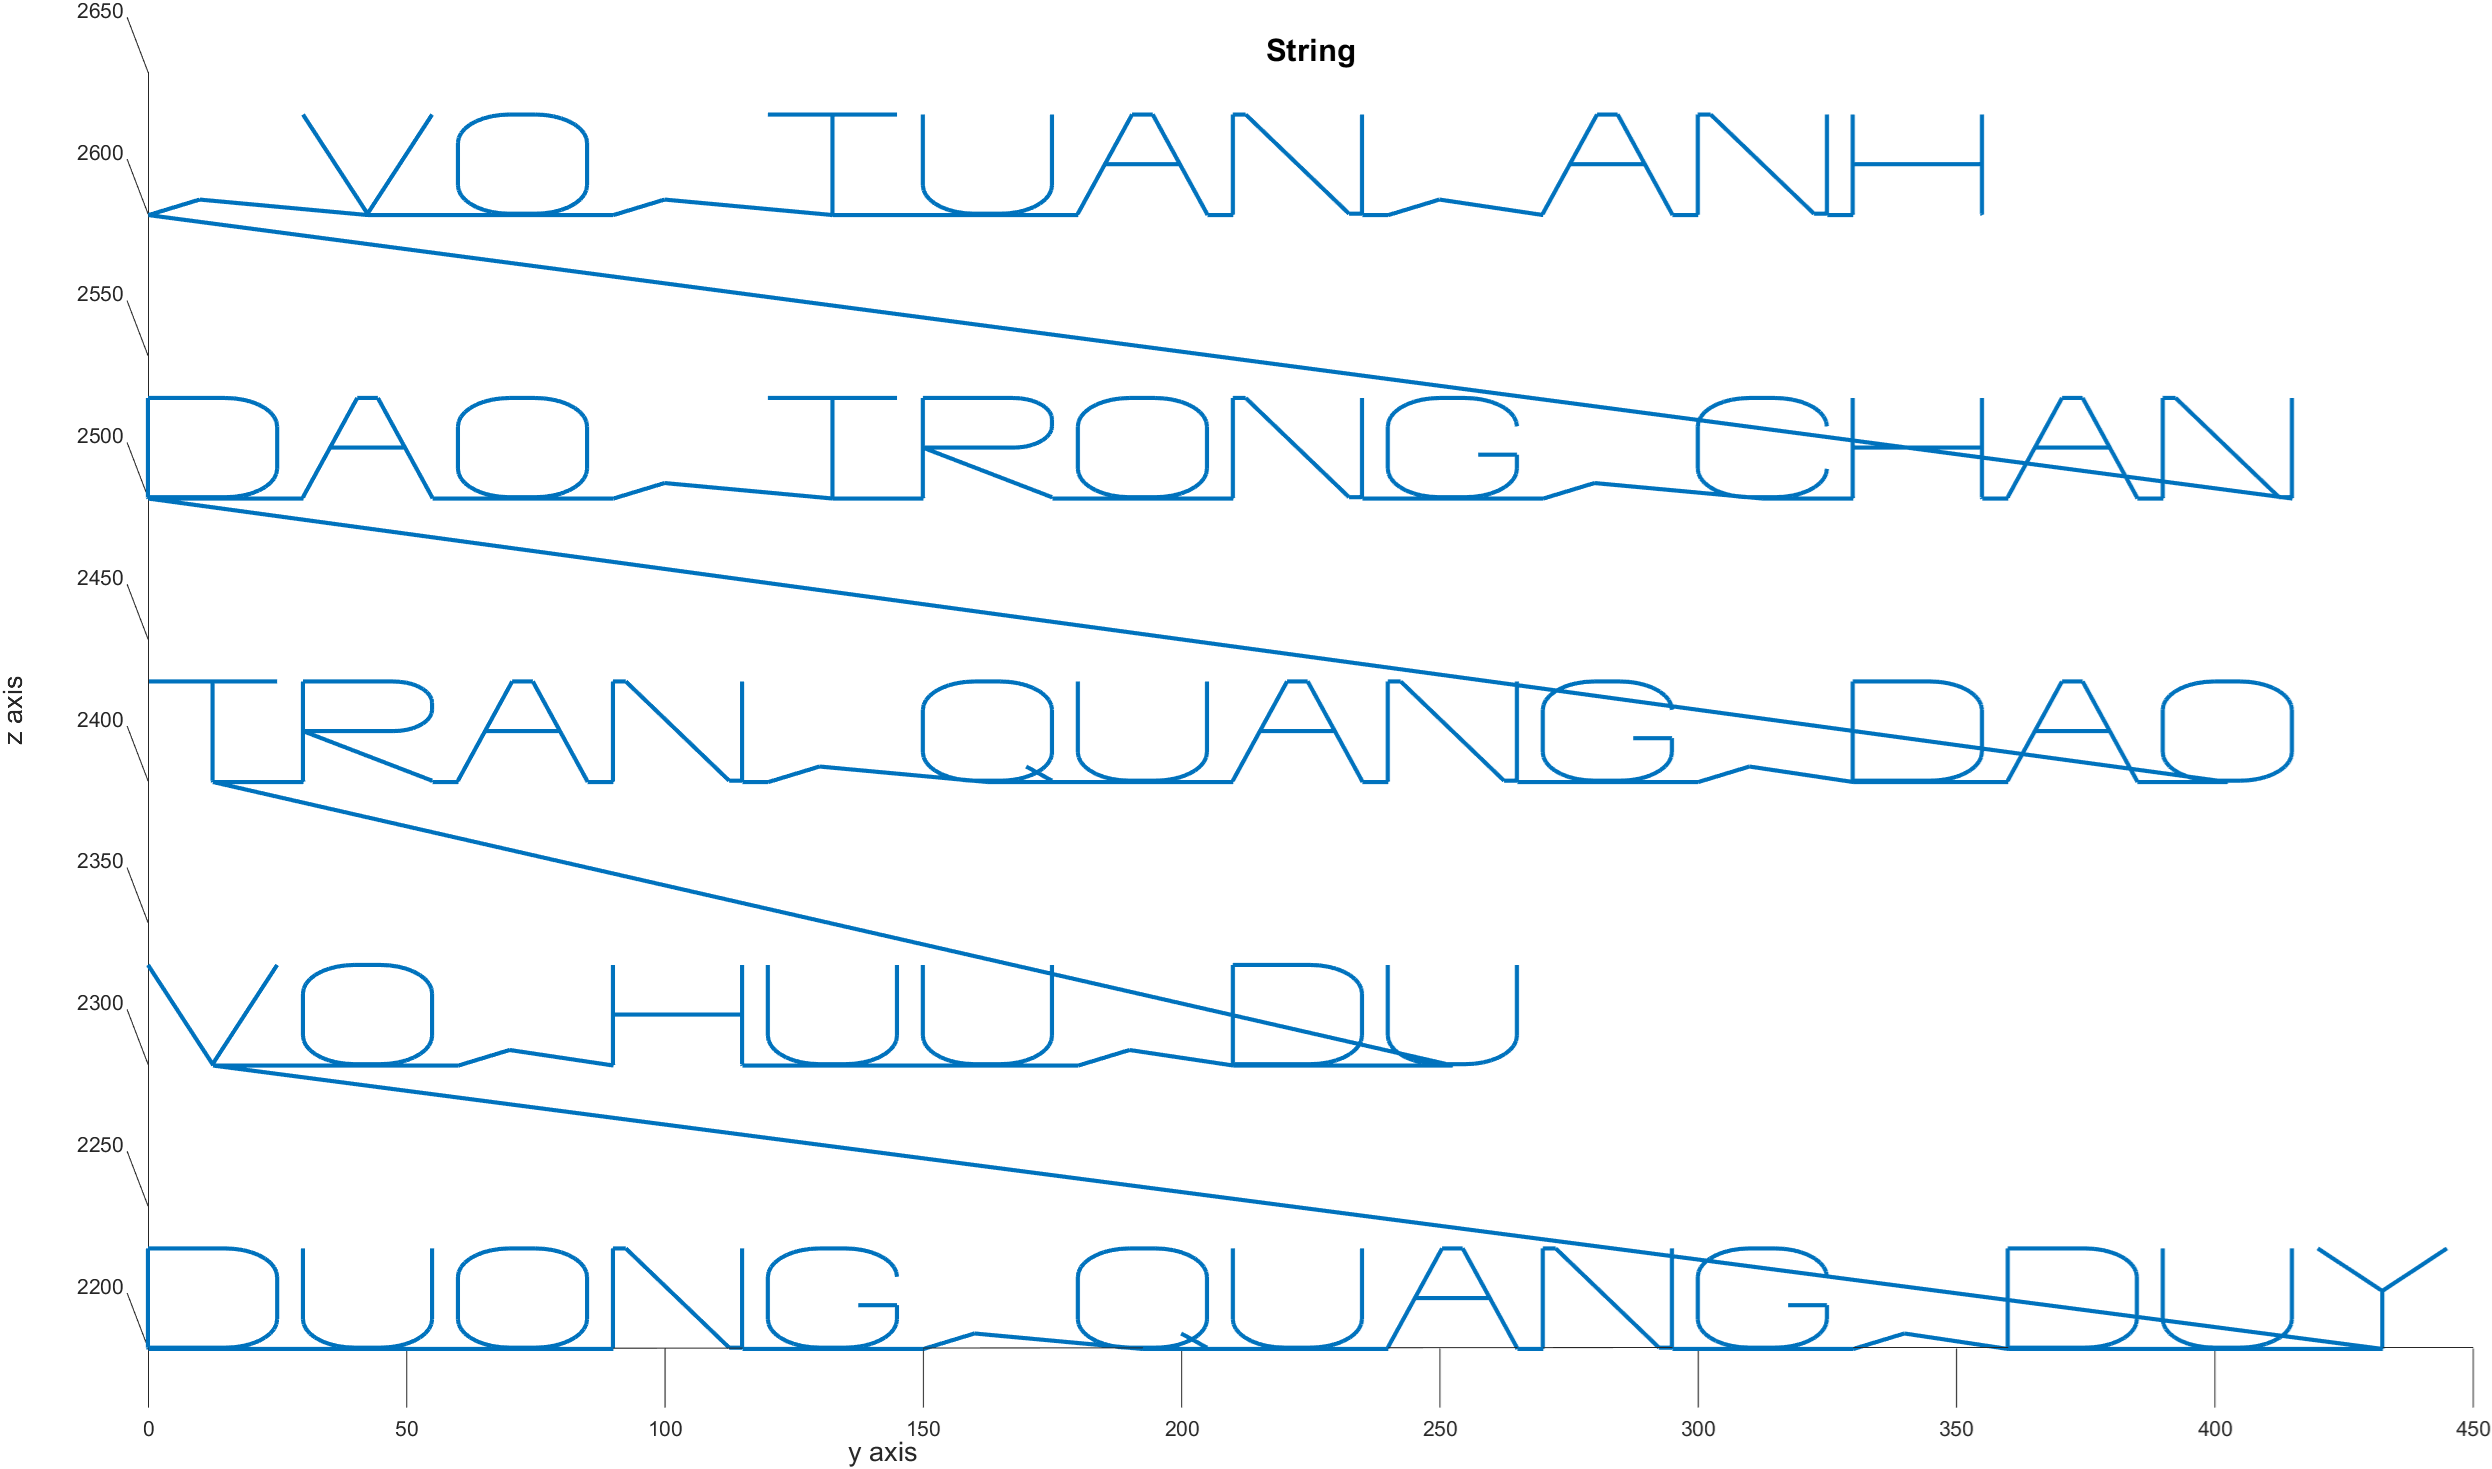
\includegraphics[width=0.8\textwidth]{pictures/result_yz.png}
        \caption{Result on YZ plane}
        \label{fig:yz_plane}
    \end{figure}